\documentclass[10pt]{article}
\usepackage[margin=0.8in]{geometry}
\usepackage{times}
\usepackage{graphicx}
\usepackage{hyperref}
\usepackage{amsmath}
\usepackage{enumitem}
\usepackage{booktabs}
\usepackage{caption}
\setlength{\parskip}{0.5em}
\setlength{\parindent}{0em}

\begin{document}

\begin{center}
{\Large \textbf{Advanced Deep Learning for Enhanced Peptide Identification in Proteomics}}\\[0.5em]
Vignesh Babu J S \& Saranath P\\[0.5em]

\end{center}



\section*{Introduction and Motivation}
Peptide identification via mass spectrometry is central to proteomics and impacts clinical diagnostics and therapeutic research. Despite advancements by frameworks like AlphaPeptDeep \cite{AlphaPeptDeep} and Prosit \cite{PrositRef}, current methods lack:
\begin{itemize}[noitemsep]
    \item Reliable uncertainty estimates that enhance model interpretability.
    \item Rich PTM embeddings that capture complex chemical properties.
\end{itemize}
Addressing these limitations is crucial for improving identification accuracy and enabling faster, more reliable proteomic analyses.

\section*{Literature Survey}

Deep learning has revolutionized the prediction of peptide properties in proteomics, surpassing traditional methods like the iRT-calculator and ELUDE. \textbf{AlphaPeptDeep} \cite{AlphaPeptDeep} is a prime example of this progress due to its modular design and ease of use.

\subsection*{Key Features}
\begin{itemize}[noitemsep]
    \item \textbf{Rich Embedding Strategies:} 
          The framework uses detailed chemical descriptors for both amino acid sequences and post-translational modifications (PTMs), allowing generalization to complex or poorly characterized modifications.
    \item \textbf{Robust Transfer Learning:} 
          Pre-trained models can be fine-tuned on limited data from new experiments, significantly enhancing predictive performance (e.g., improvements in PCC90).
    \item \textbf{User-Friendly Model Shop:} 
          Ready-to-use templates based on LSTM, CNN, and transformer architectures simplify the development and customization of deep learning models.
\end{itemize}

\section*{Research Gap}
Although significant progress has been made with methods such as AlphaPeptDeep and Prosit, several key challenges remain unaddressed:
\begin{enumerate}[noitemsep]
    \item Existing methods do not yet provide robust confidence intervals for predictions, which limits model interpretability.
    \item Detailed chemical descriptors for PTM embedding are not fully leveraged in current approaches.
    \item There is a lack of real-time inference capabilities on resource-constrained devices.
    \item Integration of sequence data with structural insights is still not comprehensively implemented.
\end{enumerate}
Our approach aims to tackle these gaps by further enhancing uncertainty quantification, improving PTM embedding quality, and exploring multi-modal integration strategies.



\section*{Project Objectives \& Methodology}

\noindent\textbf{Thread A: Uncertainty \& Interpretability.} We will integrate Monte Carlo dropout and deep ensembles into our RT/MS\textsuperscript{2} models to generate prediction distributions and confidence intervals, then benchmark PICP and calibration curves against deterministic baselines.

\medskip
\noindent\textbf{Thread B: PTM Embedding.} By augmenting the existing PTM vector with molecular weight, hydrophobicity and polarity—and applying an attention layer to weight these features contextually—we aim to boost spectral‐prediction accuracy, assessed via Pearson correlation improvements.

\medskip
\noindent\textbf{Thread C: Multi‑Modal Fusion.} Sequence embeddings will be fused with structural features (secondary structure, solvent accessibility from AlphaFold) to enhance RT/MS\textsuperscript{2} predictions, with gains quantified against sequence‐only models.


\section*{Expected Outcomes and Evaluation Strategy}
\textbf{Outcomes:}
\begin{itemize}[noitemsep]
    \item Models with robust uncertainty quantification offering reliable confidence intervals.
    \item Enhanced spectral predictions through enriched PTM embeddings.

\end{itemize}
\textbf{Evaluation:}
\begin{itemize}[noitemsep]
    \item Use statistical metrics (Pearson correlation, R\textsuperscript{2}, and PICP) for benchmarking.
    \item Compare against current state-of-the-art methods to assess improvements.
\end{itemize}


\section*{Timeline (1.5 Months)}
\begin{tabular}{@{}ll@{}}
\toprule
\textbf{Week} & \textbf{Milestones} \\ \midrule
1 & Literature review, dataset acquisition, and baseline experiments \\
2 & Implement and test Thread A (Uncertainty Quantification) \\
3 & Develop and integrate Thread B (Enhanced PTM Embedding) \\
4 & Preliminary benchmarking and refinement of Threads A \& B \\
5 & Explore structural feature extraction (Thread C) \\
6 & Final evaluations, documentation, and preparation of deliverables \\ \bottomrule
\end{tabular}

\section*{Preliminary Results and Preparatory Work}
Initial experiments using the AlphaPeptDeep framework \cite{AlphaPeptDeep} have achieved MS2 predictions with Pearson correlations exceeding 90\% and RT model fine-tuning that improves R\textsuperscript{2} from 0.93 to above 0.98. These promising results validate our planned improvements. We have access to GPU clusters, and our implementation will use Python with PyTorch. A GitHub repository will host the code along with thorough documentation.
\section*{Results Summary: Thread A}

\noindent\textbf{Overview:}  
Experiments on RT and MS2 uncertainty were conducted using the dataset available \href{https://www.ebi.ac.uk/pride/archive/projects/PXD004732}{here}.

\medskip
\noindent\textbf{RT Predictions:}  
The RT model shows a high mean absolute error ($\approx$32.68) and very low PICP ($\approx$2.1\%), indicating overconfident, narrow intervals. MC dropout and ensemble methods yield MPIW values of $\approx$0.1905 and $\approx$0.2464, respectively, but both share the same low PICP, suggesting the need for additional calibration or data.

\medskip
\noindent\textbf{MS2 Predictions:}  
While the model predicts plausible fragment spectra, MC dropout gives meaningful uncertainty estimates (Intensity $\approx$0.0313, b-ion $\approx$0.0300, y-ion $\approx$0.0326). In contrast, ensemble uncertainties are near machine precision ($\sim10^{-10}$), reflecting insufficient diversity.

\medskip
\noindent\textbf{Summary Table:}
\begin{center}
\begin{tabular}{lccc}
\toprule
\textbf{Method} & \textbf{Metric} & \textbf{RT Value} & \textbf{MS2 (Intensity)} \\
\midrule
MC Dropout & PICP   & 0.0213 & -- \\
MC Dropout & MPIW   & 0.1905 & 0.0313 \\
Ensemble   & PICP   & 0.0213 & -- \\
Ensemble   & MPIW   & 0.2464 & $\sim 0$ \\
\bottomrule
\end{tabular}
\end{center}

\subsubsection*{Visual Summaries}
\begin{figure}[htbp]
\centering
% First row
\begin{minipage}[b]{0.4\textwidth}
    \centering
    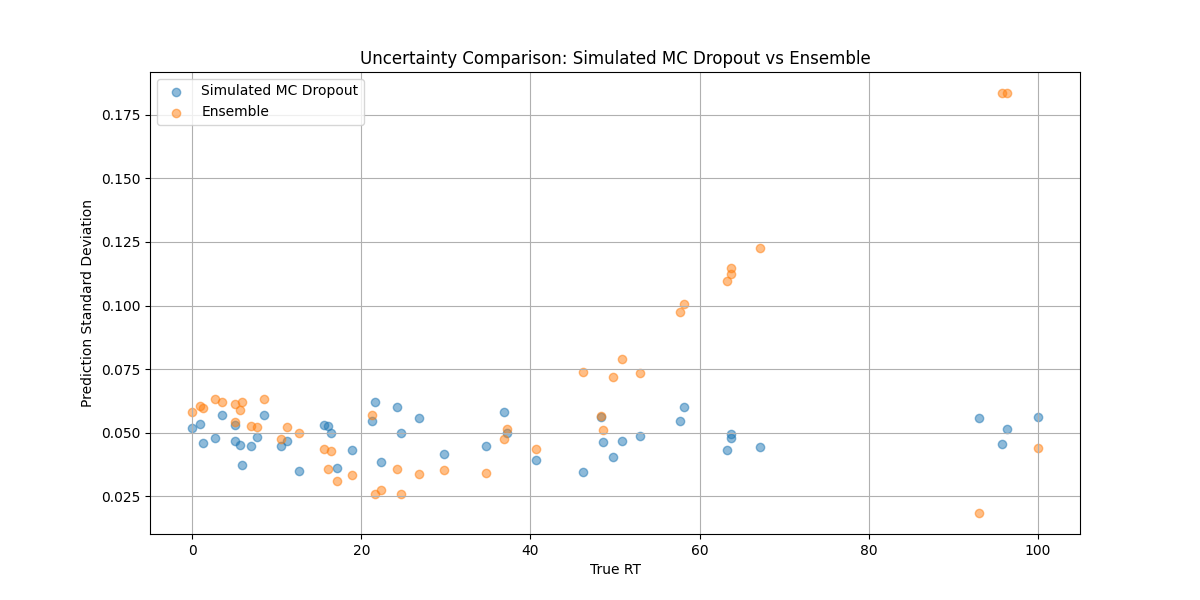
\includegraphics[width=\textwidth]{uncertainty_comparison.png}
    \captionof{figure}{Overall Uncertainty Comparison between Methods.}
    \label{fig:uncertainty_comparison}
\end{minipage}\hfill
\begin{minipage}[b]{0.4\textwidth}
    \centering
    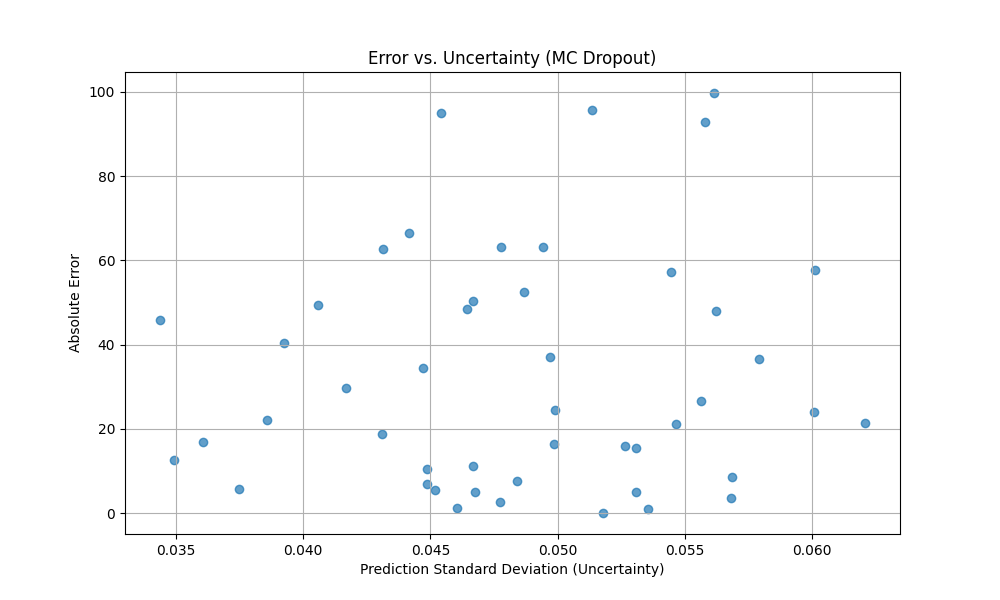
\includegraphics[width=\textwidth]{mc_dropout_error_vs_uncertainty.png}
    \captionof{figure}{Error vs. Uncertainty (MC Dropout).}
    \label{fig:mc_dropout_error}
\end{minipage}

\vspace{1em}
% Second row
\begin{minipage}[b]{0.4\textwidth}
    \centering
    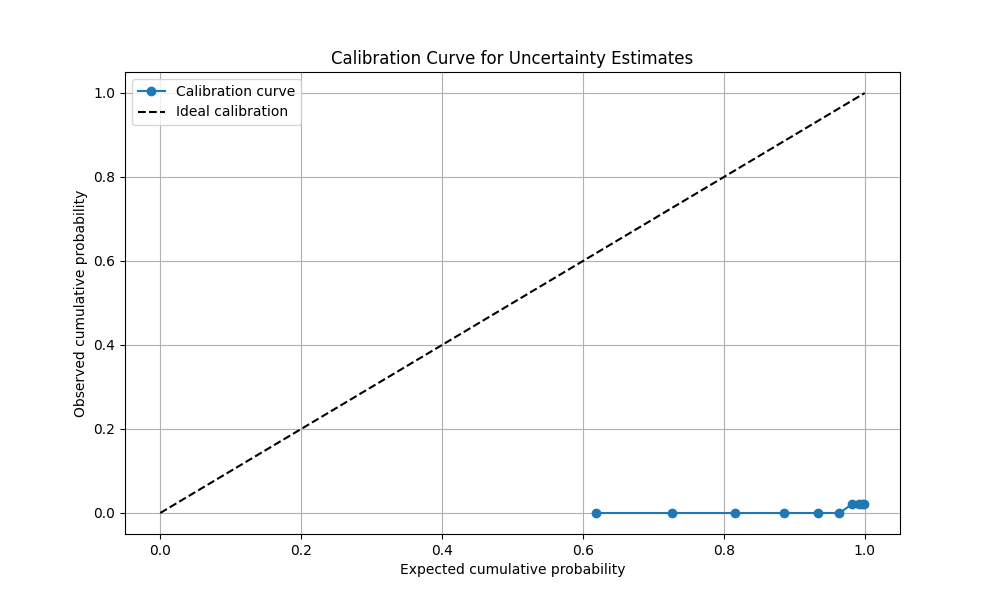
\includegraphics[width=\textwidth]{ensemble_calibration.png}
    \captionof{figure}{Ensemble Calibration Plot.}
    \label{fig:ensemble_calibration}
\end{minipage}\hfill
\begin{minipage}[b]{0.4\textwidth}
    \centering
    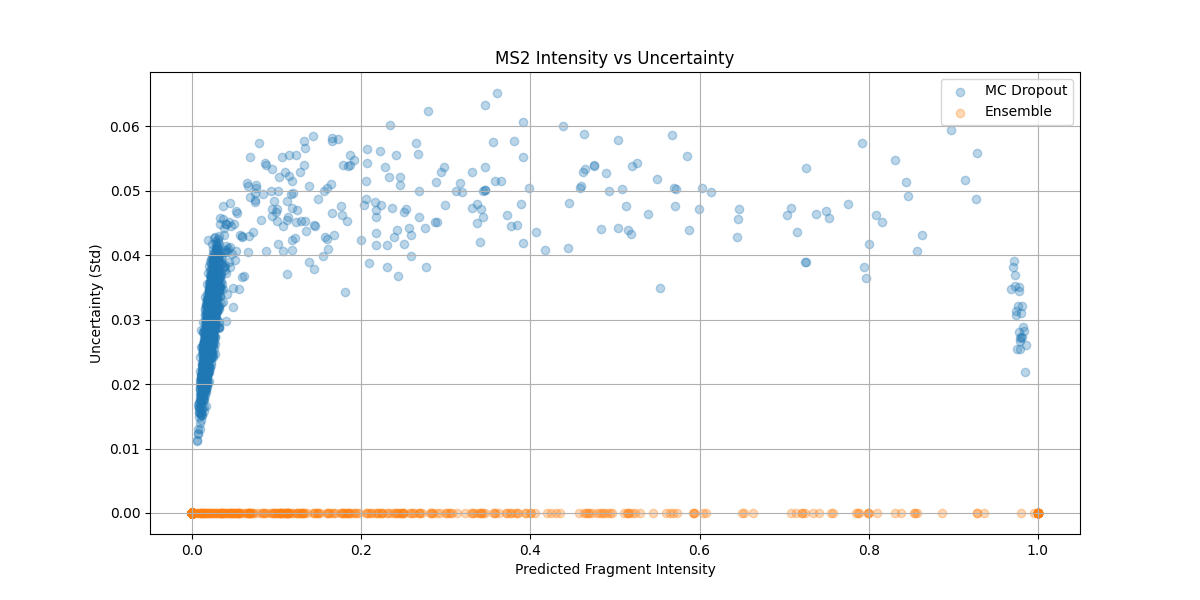
\includegraphics[width=\textwidth]{ms2_intensity_vs_uncertainty.png}
    \captionof{figure}{MS2 Intensity vs. Uncertainty.}
    \label{fig:ms2_intensity}
\end{minipage}

\vspace{1em}
% Third row
\begin{minipage}[b]{0.4\textwidth}
    \centering
    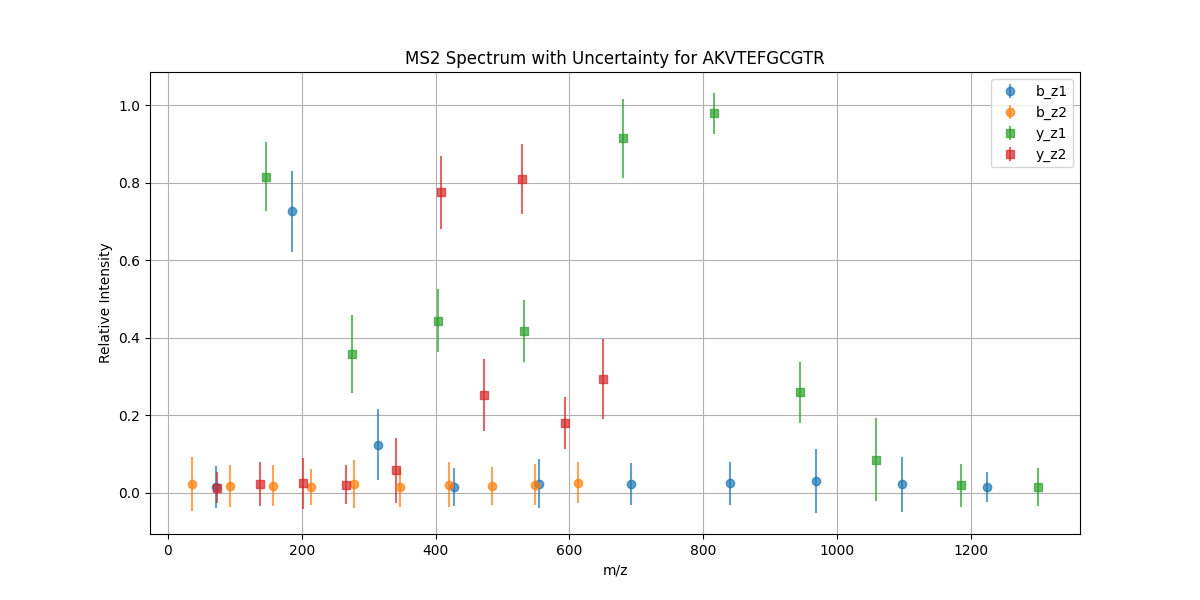
\includegraphics[width=\textwidth]{mc_dropout_ms2_uncertainty_AKVTEFGCGTR.png}
    \captionof{figure}{MC Dropout MS2 Uncertainty for Peptide AKVTEFGCGTR.}
    \label{fig:mc_dropout_ms2}
\end{minipage}\hfill
\begin{minipage}[b]{0.4\textwidth}
    \centering
    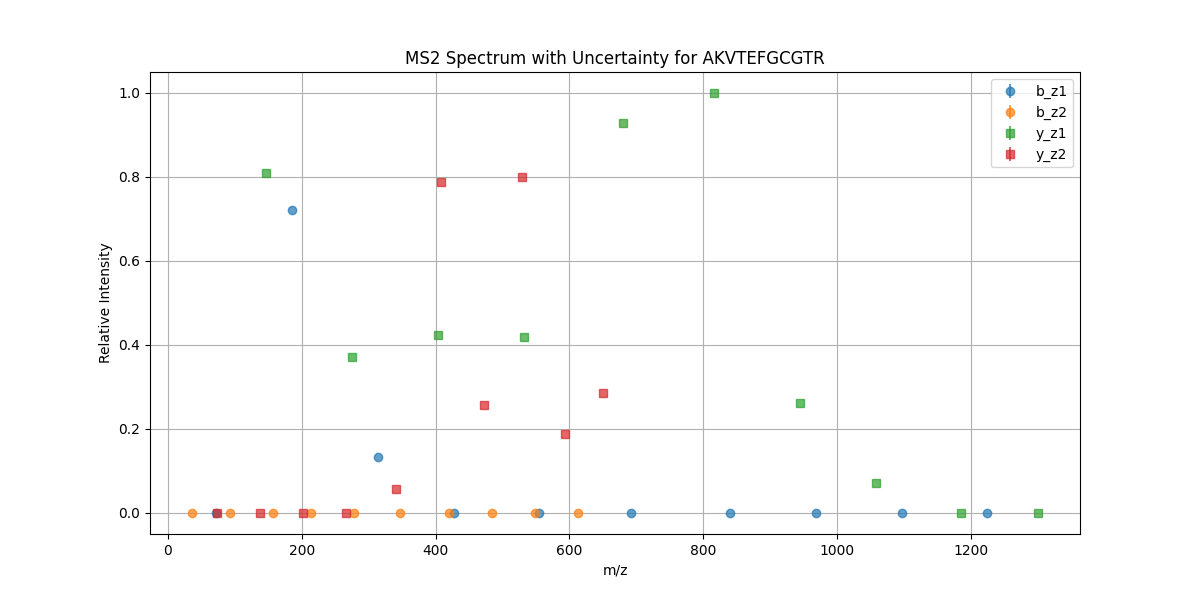
\includegraphics[width=\textwidth]{ensemble_ms2_uncertainty_AKVTEFGCGTR.png}
    \captionof{figure}{Ensemble MS2 Uncertainty for Peptide AKVTEFGCGTR.}
    \label{fig:ensemble_ms2}
\end{minipage}
\end{figure}


\subsubsection*{Conclusions and Next Steps}
\begin{itemize}[noitemsep]
    \item \textbf{RT Model:}  
    The substantial underestimation in uncertainty (low PICP, high absolute error) signals that additional data, retraining, and calibration adjustments are required.
    \item \textbf{MS2 Predictions:}  
    The MC dropout method yields interpretable uncertainties correlated with fragment intensity predictions. The ensemble method, however, needs revision to improve its diversity.
    \item \textbf{General Integration:}  
    Refining uncertainty estimates and incorporating them into downstream pipelines (e.g., confidence-weighted peptide-spectrum matches) is a priority for improving overall proteomic reliability.
\end{itemize}

\vspace{1em}

\section*{Conclusion}
This work enhances proteomics by integrating robust uncertainty estimates and enriched PTM embeddings for more accurate, interpretable peptide identification. Our modular framework promises broad impact in research and clinical settings.


\end{document}
